%%%%%%%%%%%%%%%%%%%%%%%%%%%%%%%%%%%%%%%%%%%%%%%%%%%%%%%%%%%%%%%%%%%%%%
% Overleaf (WriteLaTeX) Example: Molecular Chemistry Presentation
%
% Source: http://www.overleaf.com
%
% In these slides we show how Overleaf can be used with standard 
% chemistry packages to easily create professional presentations.
% 
% Feel free to distribute this example, but please keep the referral
% to overleaf.com
% 
%%%%%%%%%%%%%%%%%%%%%%%%%%%%%%%%%%%%%%%%%%%%%%%%%%%%%%%%%%%%%%%%%%%%%%

\documentclass{beamer}

\mode<presentation>
{
  \usetheme{Madrid}       % or try default, Darmstadt, Warsaw, ...
  \usecolortheme{default} % or try albatross, beaver, crane, ...
  \usefonttheme{default}    % or try default, structurebold, ...
  \setbeamertemplate{navigation symbols}{}
  \setbeamertemplate{caption}[numbered]
} 

\usepackage[english]{babel}
\usepackage[utf8x]{inputenc}
\usepackage{graphicx}
\usepackage{hyperref}
  \hypersetup{colorlinks=true}
  \hypersetup{urlcolor=blue}
  \hypersetup{linkcolor = .}
\usepackage{xcolor}
\usepackage{siunitx}
  \sisetup{separate-uncertainty = true}
\usepackage{physics}
\usepackage[font=small,labelfont=bf,justification=centering]{caption}
\usepackage{subcaption}
\usepackage[en-GB]{datetime2}
\usepackage{overpic}
\usepackage{feynmp}
\DeclareGraphicsRule{*}{mps}{*}{}
\usepackage{scalerel}
\newcommand{\mylbrace}[2]{\vspace{#2pt}\hspace{6pt}\scaleleftright[\dimexpr5pt+#1\dimexpr0.06pt]{\lbrace}{\rule[\dimexpr2pt-#1\dimexpr0.5pt]{-4pt}{#1pt}}{.}}
\newcommand{\myrbrace}[2]{\vspace{#2pt}\scaleleftright[\dimexpr5pt+#1\dimexpr0.06pt]{.}{\rule[\dimexpr2pt-#1\dimexpr0.5pt]{-4pt}{#1pt}}{\rbrace}\hspace{6pt}}

% Display code
\usepackage{listings}

% Here's where the presentation starts, with the info for the title slide
\title[ARC]{ARC - a novel RICH detector for a future \texorpdfstring{$e^+e^-$}{e+e-} collider \\ARC detector implementation discussion}

\author{\textbf{Martin Tat}\inst{1}\hspace{1.1em} Roger Forty\inst{2}\hspace{1.1em} Guy Wilkinson\inst{1}}
\institute{\inst{1}University of Oxford \and \inst{2}CERN}
\date{24th October 2023}

\titlegraphic{
\includegraphics[height = 2cm]{OxfordLogo.pdf}\hspace{1cm}~%
              
\includegraphics[height = 2cm]{CERNLogo.png}}

\begin{document}

\begin{frame}
  \titlepage
\end{frame}

% These three lines create an automatically generated table of contents.
\begin{frame}{Outline}
  \tableofcontents
\end{frame}

\section{\textbf{A}rray of \textbf{R}ICH \textbf{C}ells}
\begin{frame}{\textbf{A}rray of \textbf{R}ICH \textbf{C}ells}
  \begin{center}
    {\huge \textbf{A}rray of \textbf{R}ICH \textbf{C}ells} \\~\\
    {\large Quick recap}
  \end{center}
\end{frame}

\begin{frame}{\textbf{A}rray of \textbf{R}ICH \textbf{C}ells}
  \begin{itemize}
    \setlength\itemsep{0.2em}
    \item{\textbf{A}rray of \textbf{R}ICH \textbf{C}ells (ARC): A novel RICH detector concept}
    \begin{itemize}
      \item{Compact, low-mass solution for particle ID for FCC-ee}
      \item{A large number of small RICH cells}
    \end{itemize}
    \item{Adapted to fit into the \href{https://arxiv.org/abs/1911.12230}{CLD experiment} concept, taking $10\%$ from the tracker volume}
    \begin{itemize}
      \item{Radial depth of $\SI{20}{\centi\meter}$, radius of $\SI{2.1}{\meter}$ and a length of $\SI{4.4}{\meter}$}
      \item{Aim to keep material budget below $0.1X_0$}
    \end{itemize}
    \item{Aerogel and gas radiators with a spherical mirror}
    \begin{itemize}
      \item{Aerogel also acts as thermal insulation between gas and detector}
    \end{itemize}
  \end{itemize}
  \begin{figure}
    \centering
    \begin{subfigure}{0.4\textwidth}
      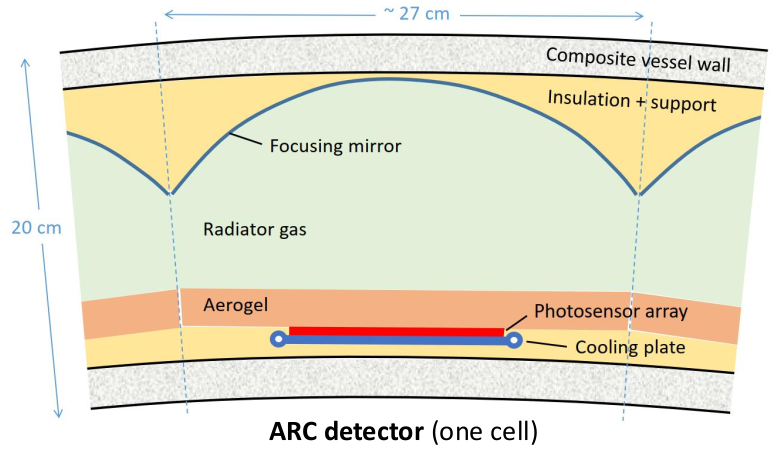
\includegraphics[width = 1.0\textwidth]{Plots/ARC_Cell.png}
    \end{subfigure}%
    \hspace{1cm}
    \begin{subfigure}{0.3\textwidth}
      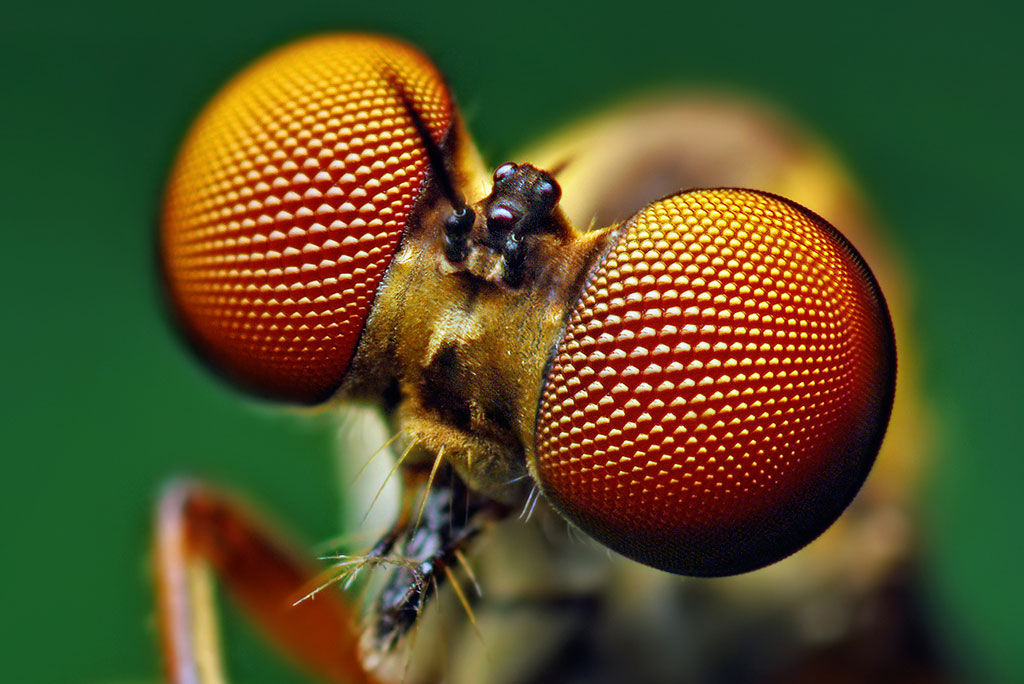
\includegraphics[width = 1.0\textwidth]{Plots/CompoundEyes.jpg}
    \end{subfigure}
    \caption{ARC has a cellular structure, similar to an insect's compound eyes}
  \end{figure}
\end{frame}

\begin{frame}{\textbf{A}rray of \textbf{R}ICH \textbf{C}ells}
  \begin{itemize}
    \setlength\itemsep{0.5em}
    \item{All cells are the same size, organised on a hexagonal grid}
    \begin{itemize}
      \item{Barrel (endcap) has $945$ ($402$) cells in total, where $18$ ($23$) are unique}
      \item{Some cells are partial cells, but all photon sensors are the same size}
    \end{itemize}
  \end{itemize}
  \begin{figure}
    \centering
    \begin{subfigure}{0.6\textwidth}
      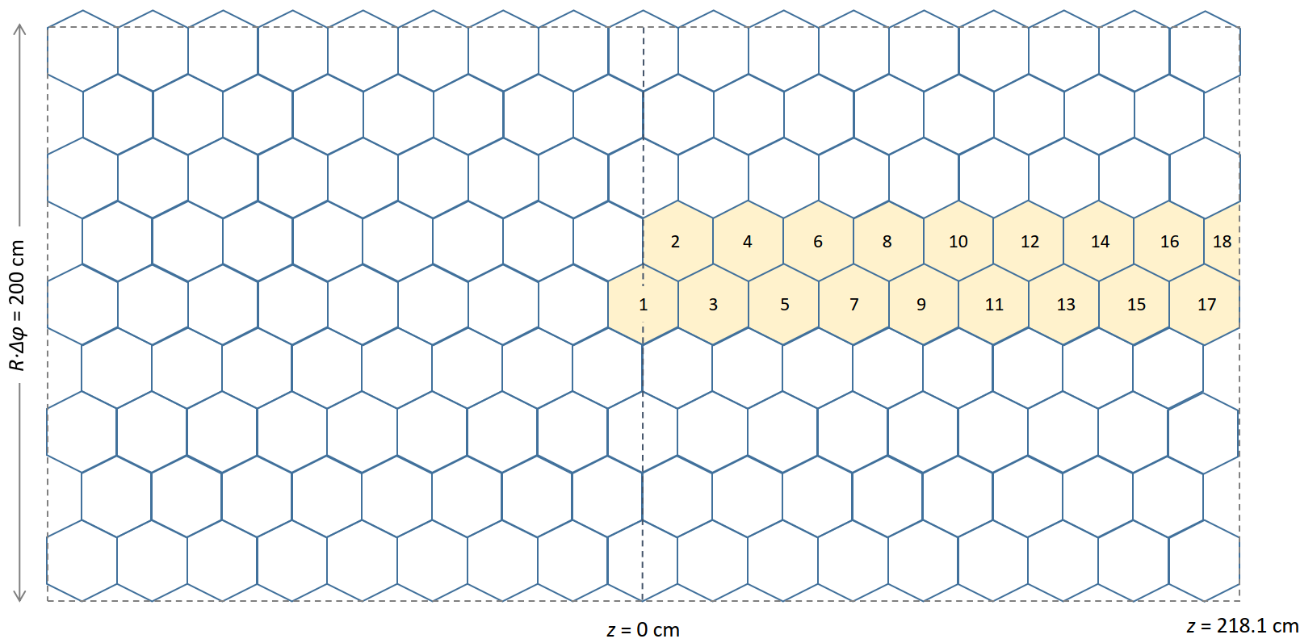
\includegraphics[width = 1.0\textwidth]{Plots/BarrelCells.png}
    \end{subfigure}%
    \begin{subfigure}{0.3\textwidth}
      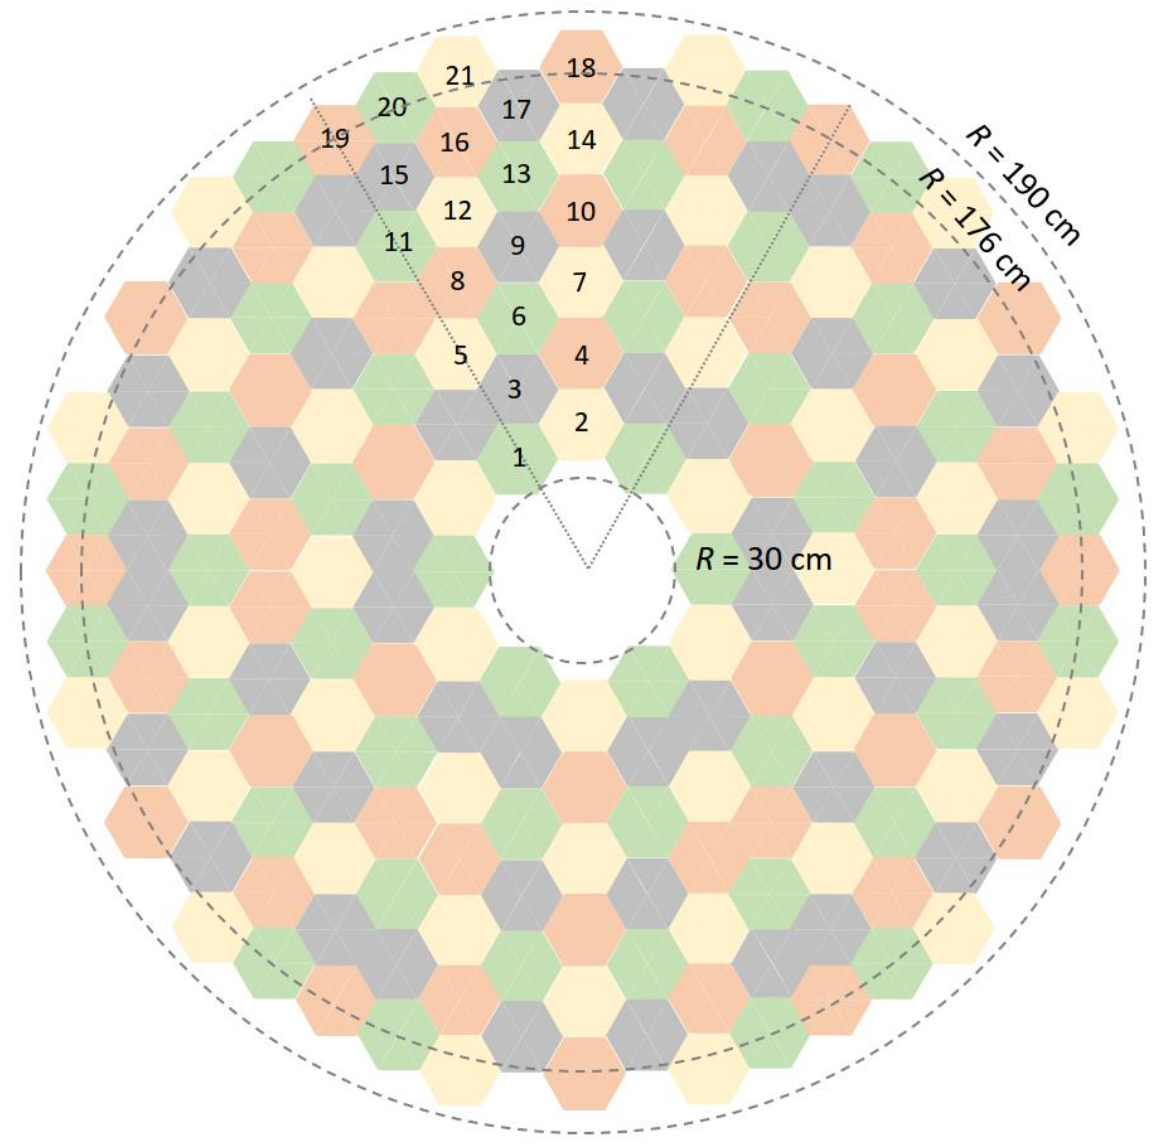
\includegraphics[width = 1.0\textwidth]{Plots/EndcapCells.png}
    \end{subfigure}
    \caption{Barrel (left) and endcap (right) cells}
  \end{figure}
\end{frame}

\begin{frame}{\textbf{A}rray of \textbf{R}ICH \textbf{C}ells}
  \begin{figure}
    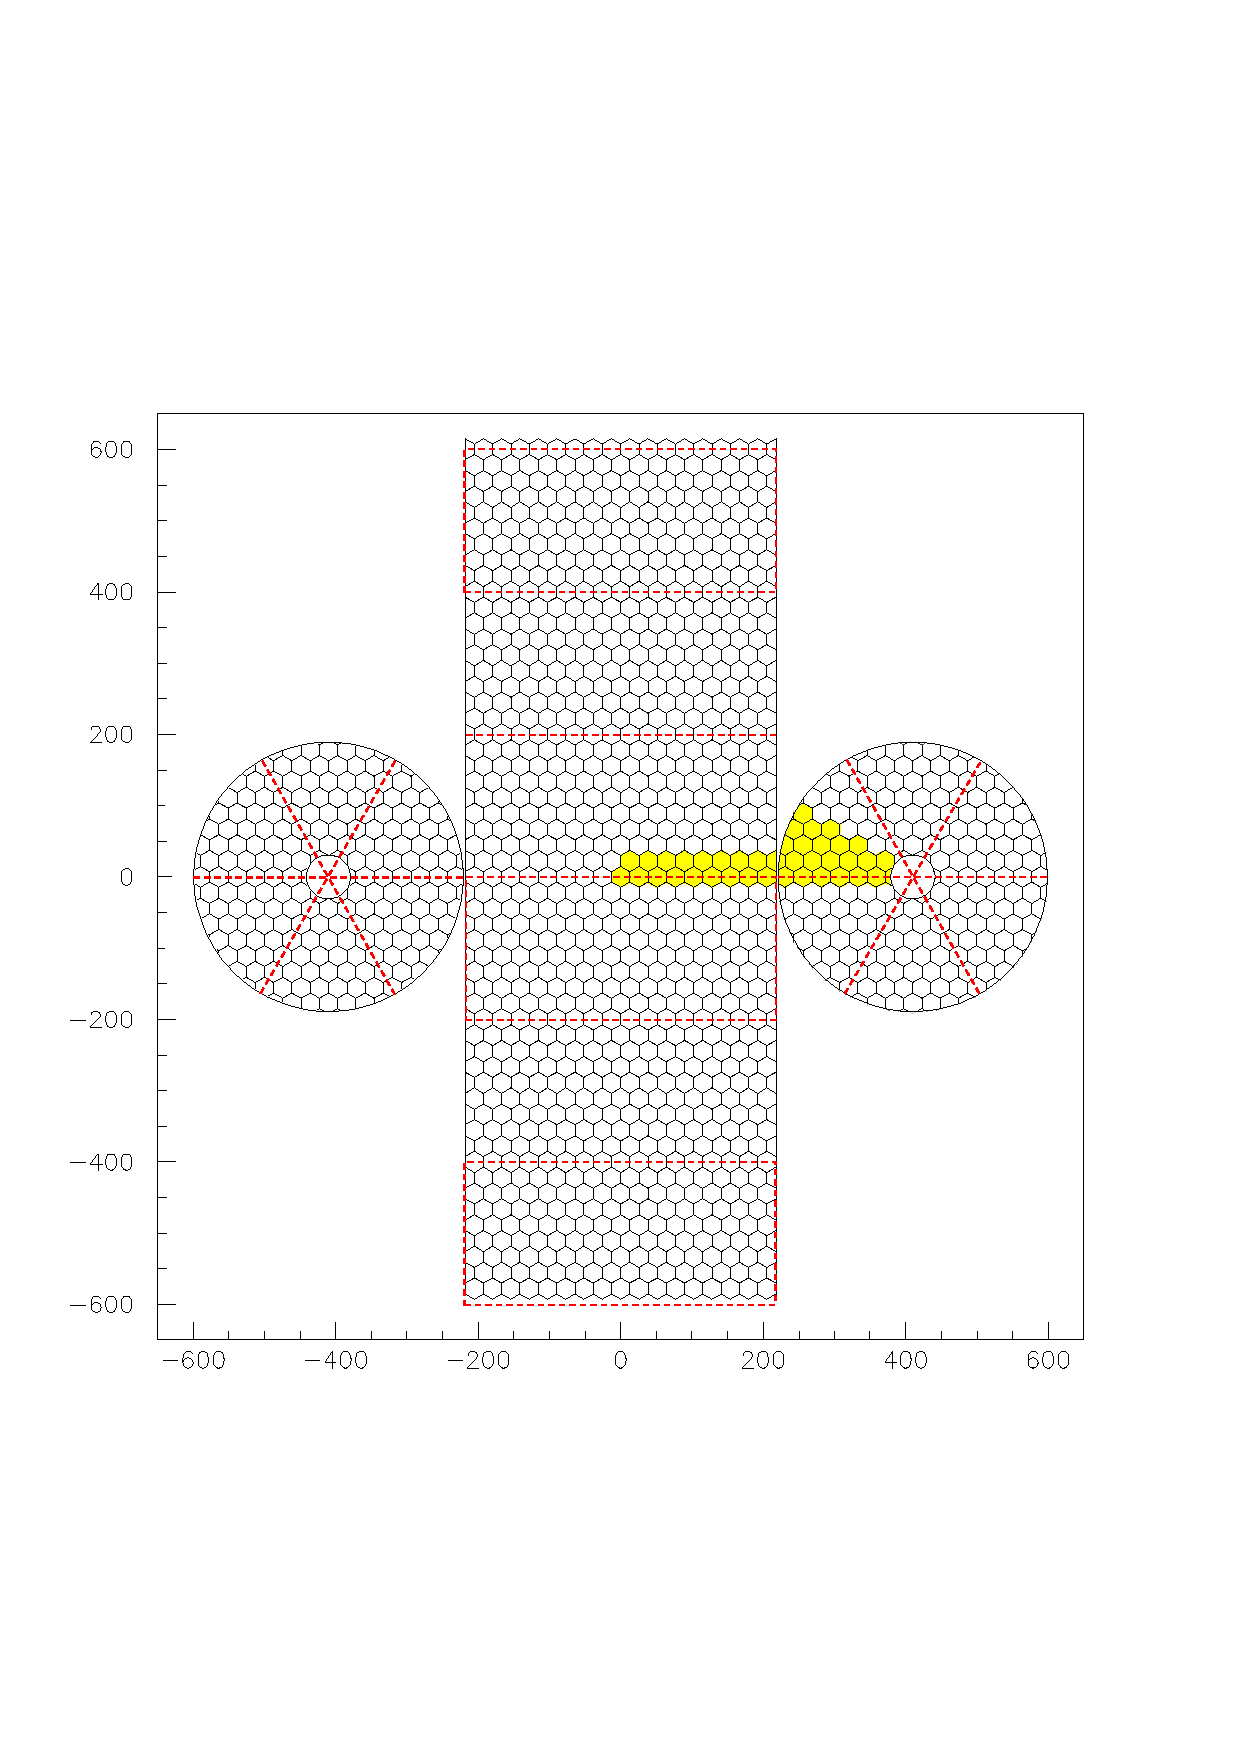
\includegraphics[width = 0.8\textwidth, trim = {0 7cm 0 7cm}, clip = true]{Plots/Display3.pdf}
    \caption{Barrel and endcap cells}
  \end{figure}
\end{frame}

\begin{frame}{Photon hits}
  \begin{figure}
    \centering
    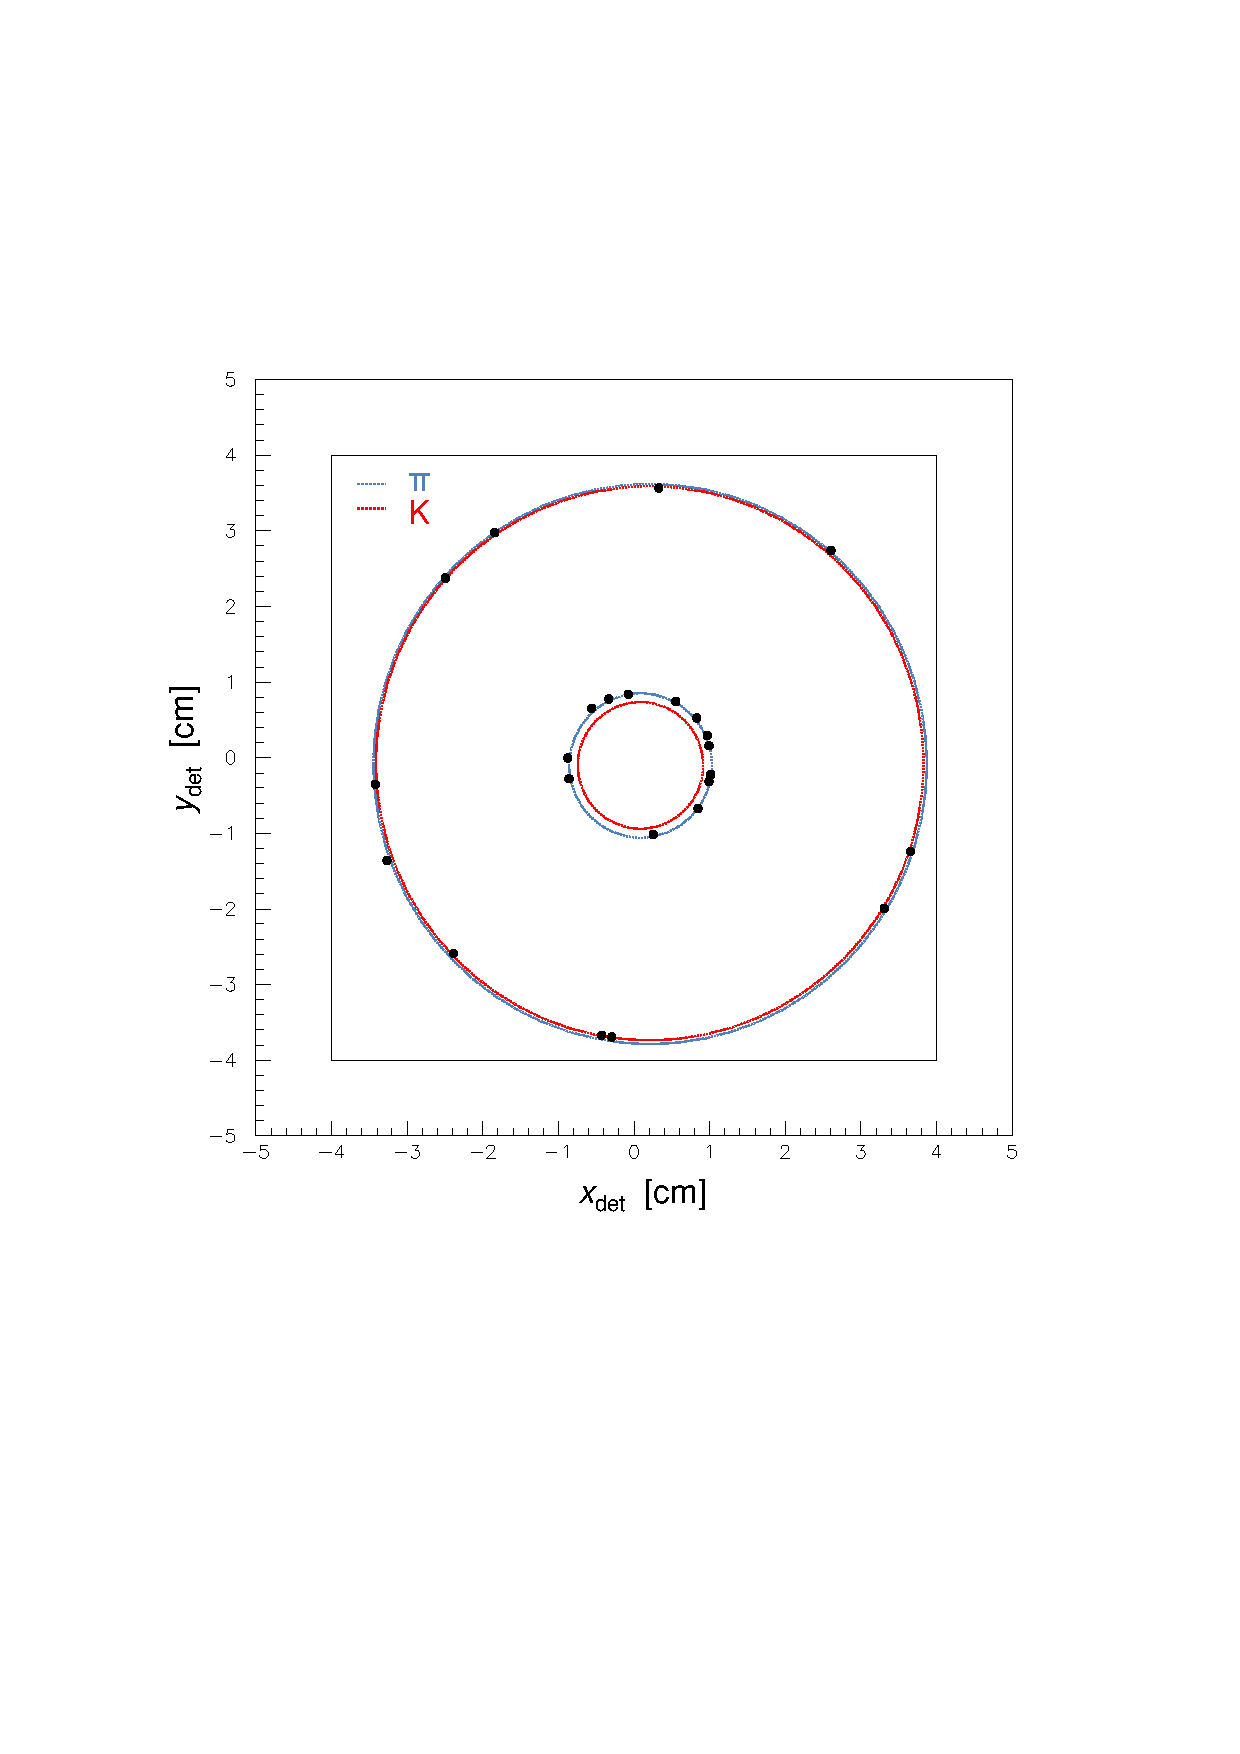
\includegraphics[width = 0.65\textwidth, trim = {2cm 9cm 3cm 6cm}, clip = true]{Plots/Display1.pdf}
    \caption{Photon hits on photodetector}
  \end{figure}
\end{frame}

\begin{frame}{Event display}
  \begin{figure}
    \centering
    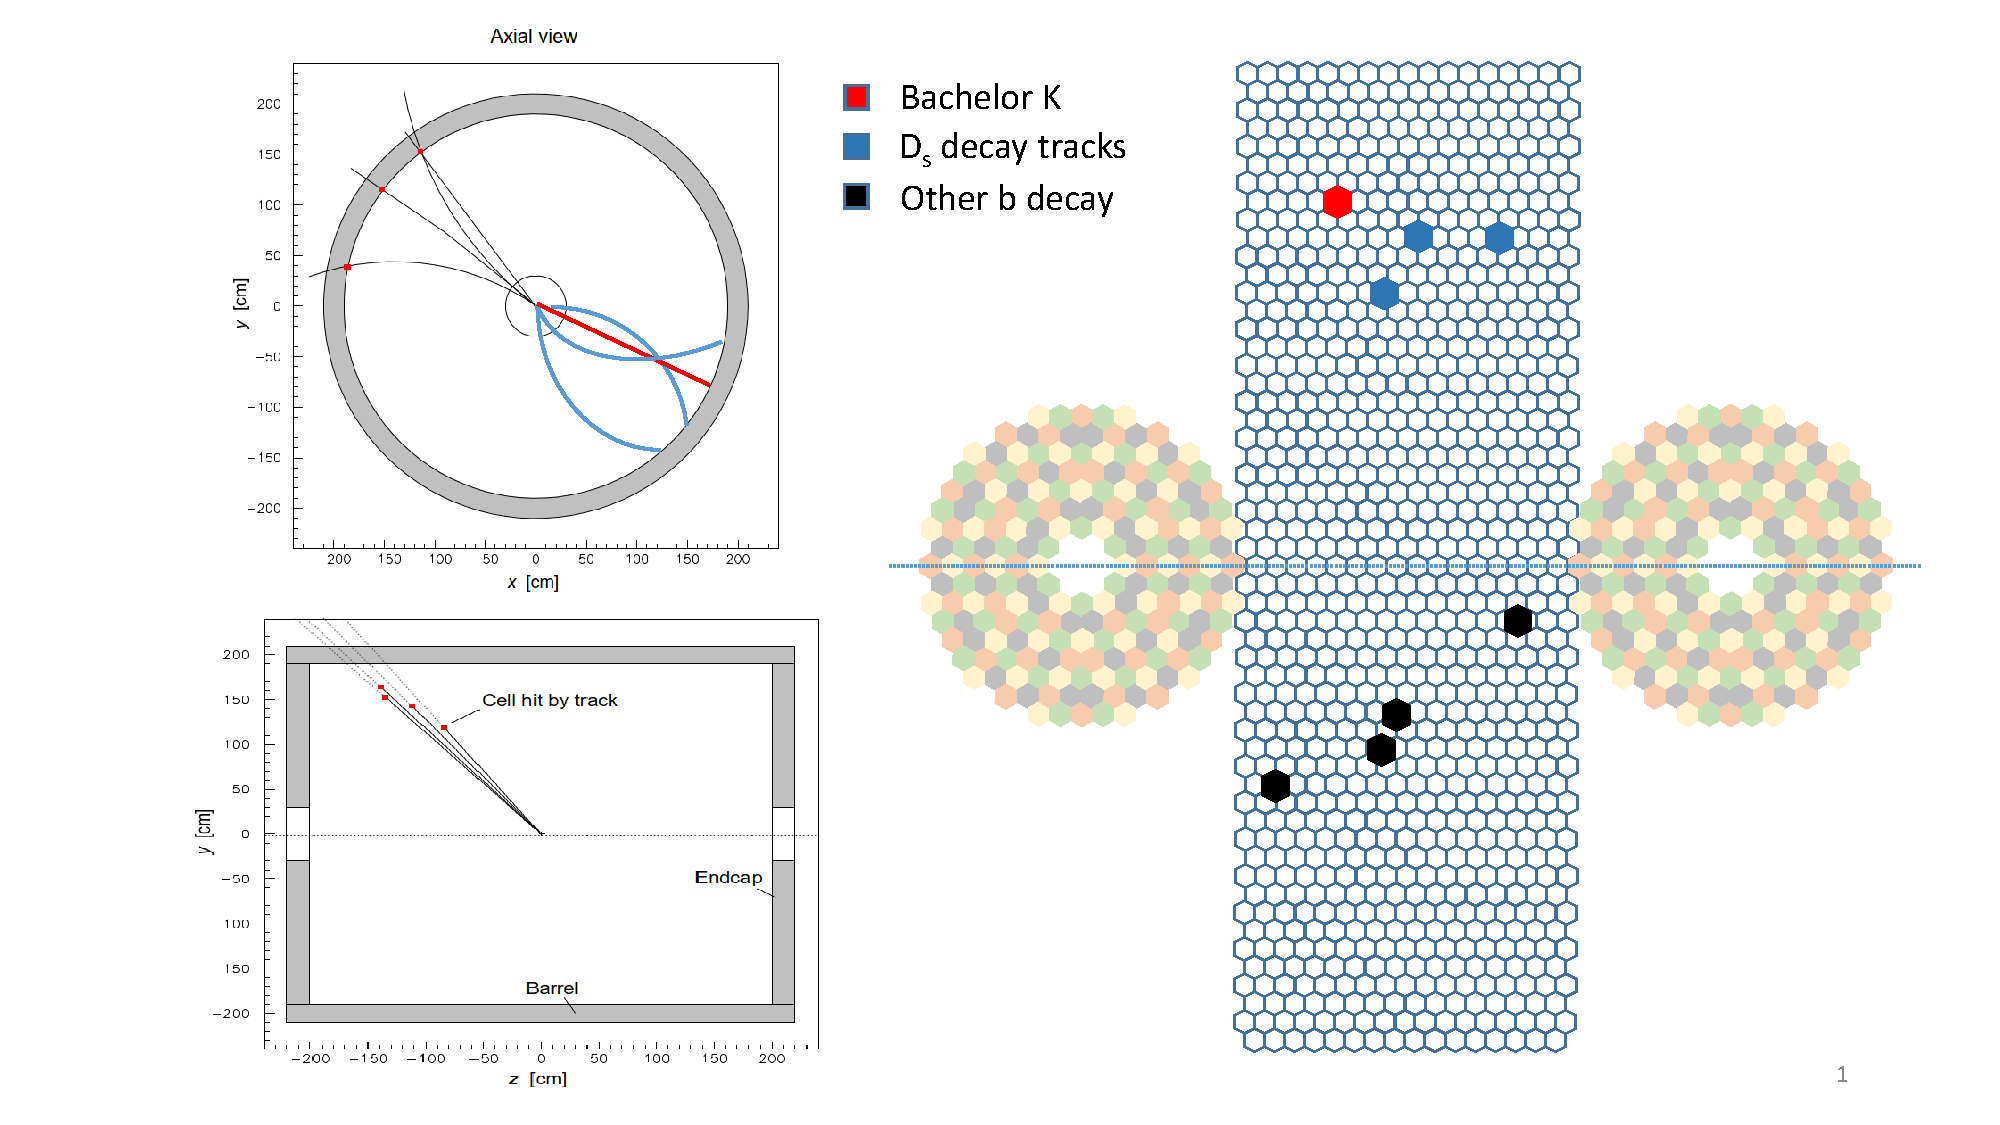
\includegraphics[width = 0.85\textwidth, trim = {0cm 2cm 0cm 0cm}, clip = true]{Plots/Display2.pdf}
    \caption{$B_s\to D_sK$}
  \end{figure}
\end{frame}

\section{Optimisation of ARC layout}
\begin{frame}{Optimisation of ARC layout}
  \begin{center}
    {\huge Optimisation of ARC layout} \\~\\
    {\large My strategy for optimising ARC}
  \end{center}
\end{frame}

\begin{frame}{How to calculate ARC performance}
  \begin{enumerate}
    \setlength\itemsep{1.0em}
    \item{Generate $2\times10^4$ charged pions with high momentum ($\SI{100}{\giga\eV}$)}
    \item{Generate Cherenkov photons from gas}
    \item{Track photons through the optics}
    \item{For each photon, reconstruct the Cherenkov angle $\theta$}
    \item{Find average $\theta$ from all detected photons from the charged track}
    \item{For each cell, vary $5$ parameters to optimise the performance}
  \end{enumerate}
  \begin{block}{``Figure of merit'': Cherenkov angle uncertainty}
    \begin{equation*}
      \Delta\theta = \frac{1}{\sqrt{N}}\times\frac{1}{N - 1}\times\sum_{i = 0}^{N - 1}(\theta - \bar{\theta})^2
    \end{equation*}
  \end{block}
\end{frame}

\begin{frame}{Parameters to optimise}
  \begin{enumerate}
    \setlength\itemsep{0.2em}
    \item{Mirror curvature}
    \item{Mirror horizontal position}    
    \item{Mirror vertical position}
    \item{Detector horizontal position}
    \item{Detector tilt}
  \end{enumerate}
  \vspace{-0.2cm}
  \begin{figure}
    \centering
    \begin{subfigure}{0.45\textwidth}
      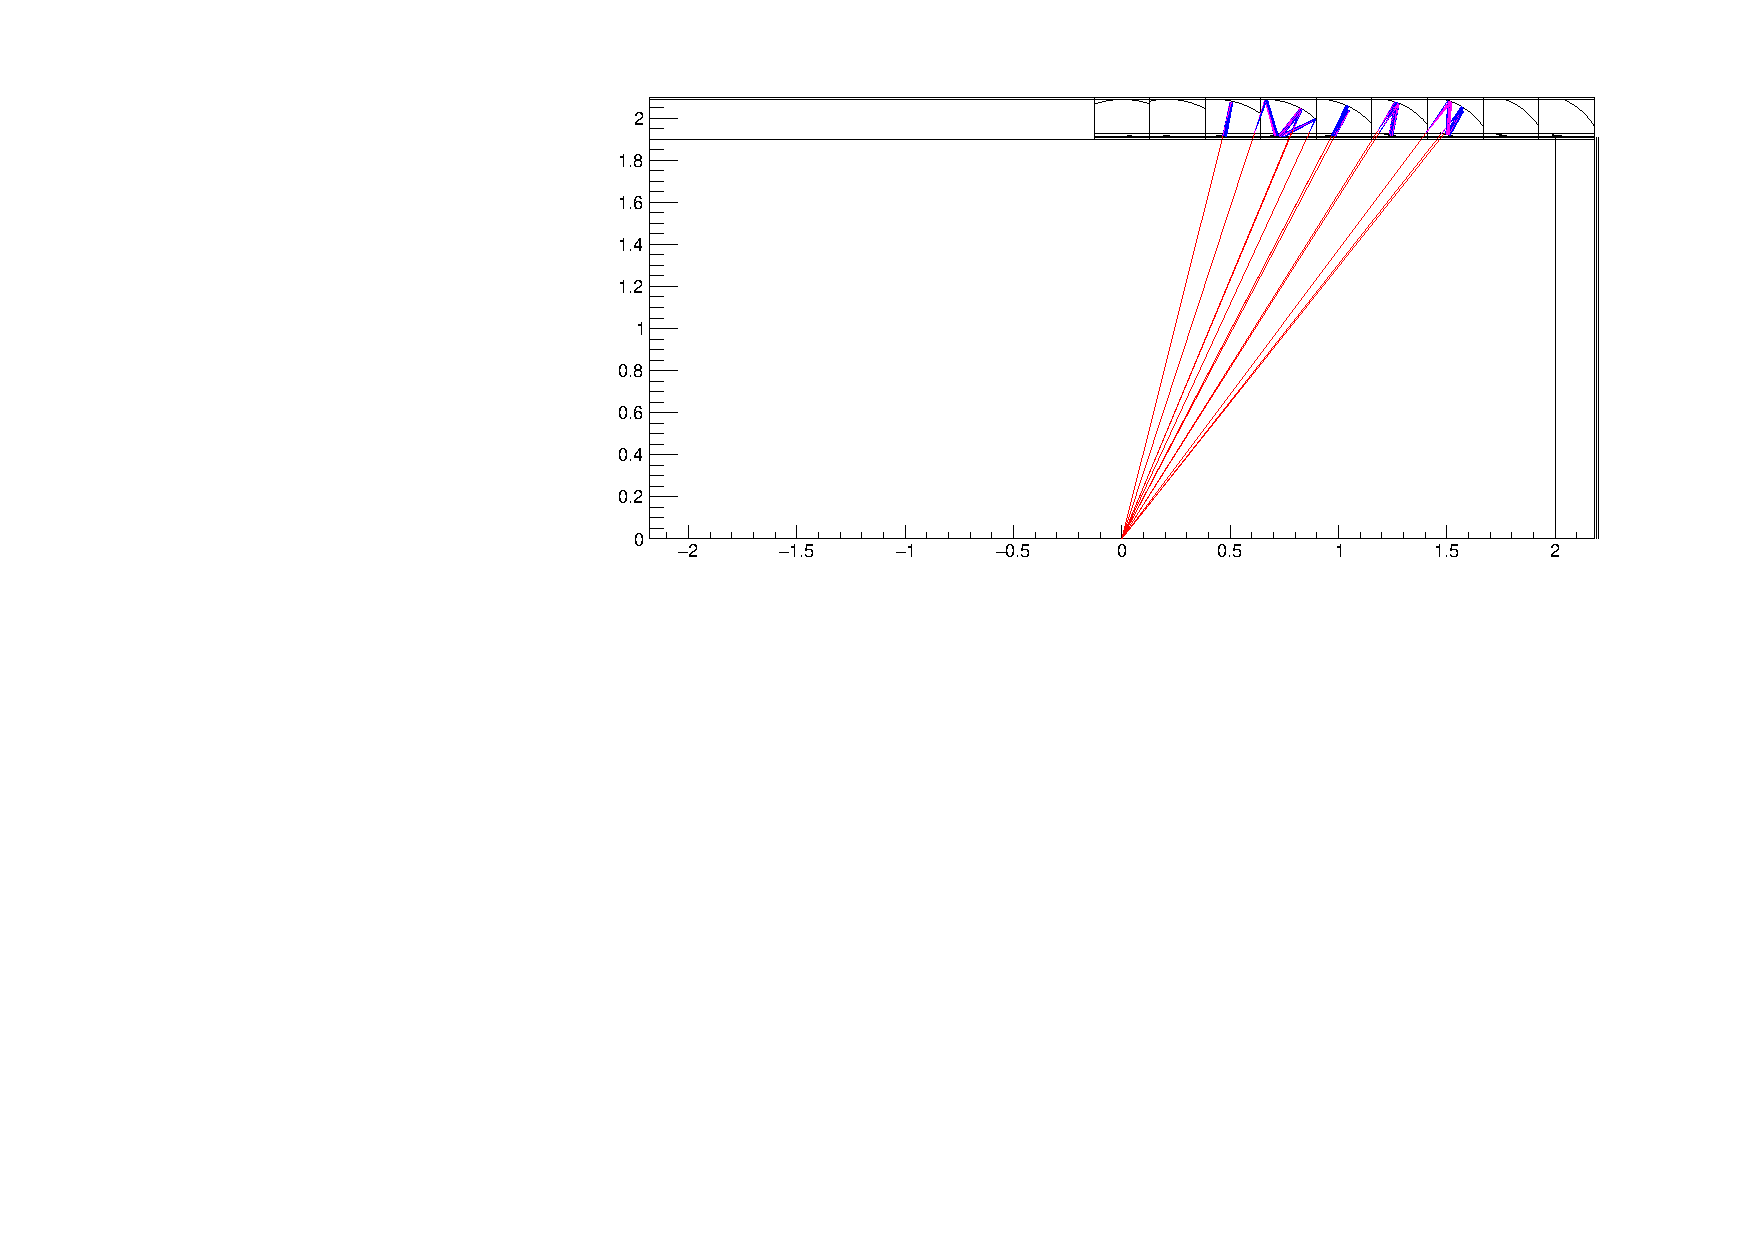
\includegraphics[width = 1.0\textwidth, trim = {11cm 5cm 3.5cm 0.5cm}, clip = true]{Plots/EventDisplay_MainRow.pdf}
    \end{subfigure}%
    \hspace{0.2cm}
    \begin{subfigure}{0.45\textwidth}
      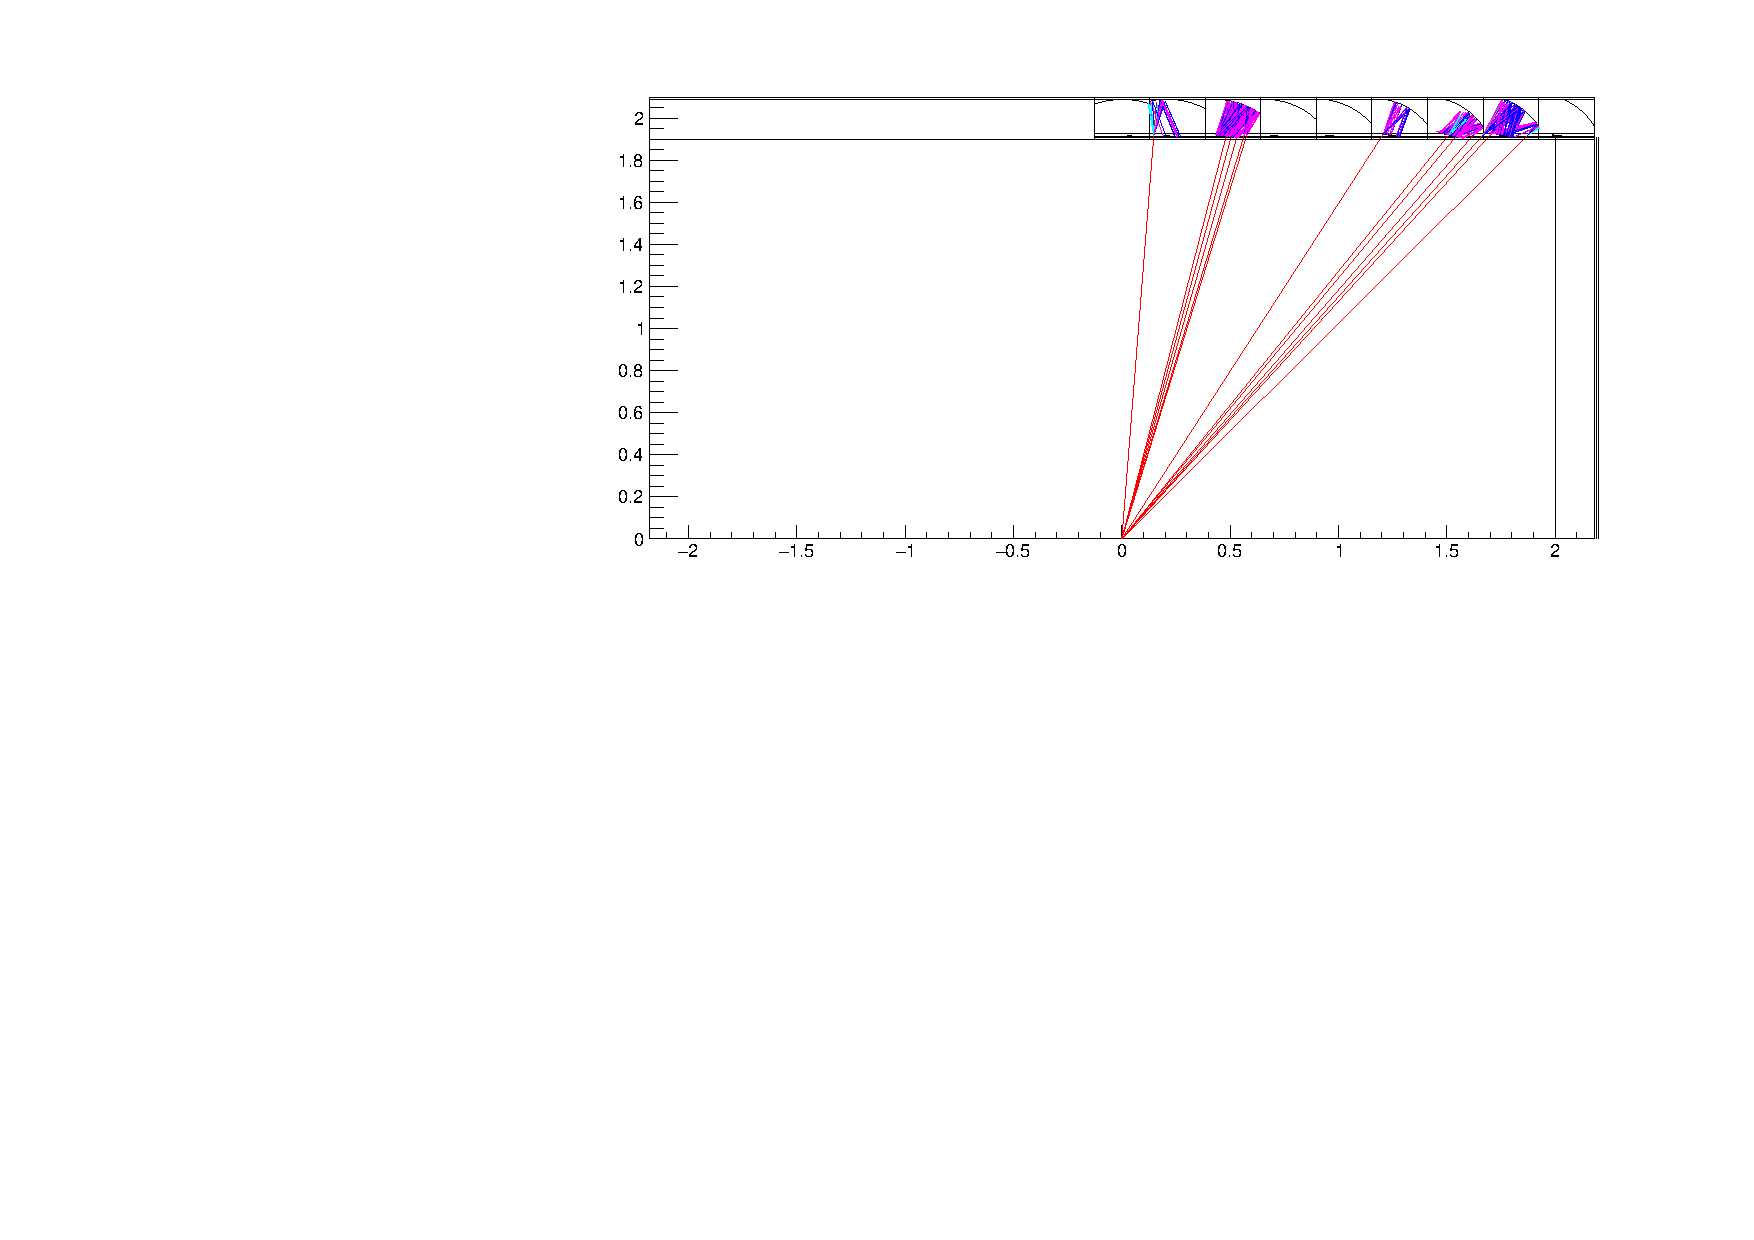
\includegraphics[width = 1.0\textwidth, trim = {11.6cm 5cm 2.9cm 0.5cm}, clip = true]{Plots/EventDisplay_MainRow_Aerogel.pdf}
    \end{subfigure}
    \caption{Tracking of photons from gas radiator (left) and aerogel radiator (right) through the ARC optics}
  \end{figure}
\end{frame}

\begin{frame}{Stochastic optimisation}
  \begin{itemize}
    \setlength\itemsep{1.0em}
    \item{Issue: Each iteration uses a finite number of photons}
    \begin{itemize}
      \item{Cannot use minimisation algorithms based on gradients}
    \end{itemize}
    \item{Use stochastic optimisation:}
    \begin{enumerate}
      \item{\href{https://en.wikipedia.org/wiki/Differential_evolution}{Differential evolution}}
      \item{Start with a population of candidate solutions in parameter space}
      \item{In each iteration, each solution has a small probability of ``evolving'' by combining existing solutions}
      \item{Iterate until it ``converges''}
    \end{enumerate}
    \item{I found an implementation \href{https://github.com/milsto/differential-evolution}{here}}
    \begin{itemize}
      \item{A bit slow, but it seems to find a sensible minimum}
      \item{Requires some tweaking of parameter bounds}
    \end{itemize}
  \end{itemize}
\end{frame}

\section{Technical details of optimisation}
\begin{frame}{Technical details of optimisation}
  \begin{center}
    {\huge Technical details of optimisation} \\~\\
    {\large How to run the code?}
  \end{center}
\end{frame}
\begin{frame}[fragile]{GitHub repository}
  \begin{center}
    My optimisation code can be found \href{https://github.com/MartinDuyTat/ARC_Simulation_Reconstruction}{here}
  \end{center}
  \begin{lstlisting}[language=bash, breaklines=true]
    git clone git@github.com:MartinDuyTat/ARC_Simulation_Reconstruction.git
    cd ARC_Simulation_Reconstruction
    mkdir build
    cd build
    cmake ..
    make install
    cd ../options
  \end{lstlisting}
  \begin{center}
    I have used ROOT 6.22/2 and C++17
  \end{center}
\end{frame}

\begin{frame}[fragile]{GitHub repository}
  \begin{center}
    To run the optimisation, we need 5 options files:
  \end{center}
  \begin{lstlisting}[language=bash, breaklines=true]
    General.txt
    ARCGeometry.txt
    RadiatorCell.txt
    Particle.txt
    Optimisation.txt
  \end{lstlisting}
  \begin{center}
    General: Number of tracks, chromatic dispersion, seed, etc
  \end{center}
\end{frame}

\begin{frame}[fragile]{GitHub repository}
  \begin{center}
    To run the optimisation, we need 5 options files:
  \end{center}
  \begin{lstlisting}[language=bash, breaklines=true]
    General.txt
    ARCGeometry.txt
    RadiatorCell.txt
    Particle.txt
    Optimisation.txt
  \end{lstlisting}
  \begin{center}
    ARCGeometry: ARC length, radius, number of cells, $B$-field strength
  \end{center}
\end{frame}

\begin{frame}[fragile]{GitHub repository}
  \begin{center}
    To run the optimisation, we need 5 options files:
  \end{center}
  \begin{lstlisting}[language=bash, breaklines=true]
    General.txt
    ARCGeometry.txt
    RadiatorCell.txt
    Particle.txt
    Optimisation.txt
  \end{lstlisting}
  \begin{center}
    RadiatorCell: Radiator size, aerogel thickness, etc, \textbf{optimised parameters}
  \end{center}
\end{frame}

\begin{frame}[fragile]{GitHub repository}
  \begin{center}
    To run the optimisation, we need 5 options files:
  \end{center}
  \begin{lstlisting}[language=bash, breaklines=true]
    General.txt
    ARCGeometry.txt
    RadiatorCell.txt
    Particle.txt
    Optimisation.txt
  \end{lstlisting}
  \begin{center}
    Particle: Momentum, particle ID, direction, etc
  \end{center}
\end{frame}

\begin{frame}[fragile]{GitHub repository}
  \begin{center}
    To run the optimisation, we need 5 options files:
  \end{center}
  \begin{lstlisting}[language=bash, breaklines=true]
    General.txt
    ARCGeometry.txt
    RadiatorCell.txt
    Particle.txt
    Optimisation.txt
  \end{lstlisting}
  \begin{center}
    Optimisation: Number of iterations, population size, bounds, etc
  \end{center}
\end{frame}

\begin{frame}[fragile]{Running the optimisation}
  \begin{center}
    To optimise cell labelled ``column $3$, row $1$'', run:
  \end{center}
  \begin{lstlisting}[language=bash, basicstyle=\tiny]
    OptimiseARC 3 1 General General.txt Particle Particle.txt \
    ARCGeometry ARCGeometry.txt RadiatorCell RadiatorCell.txt Optimisation Optimisation.txt
  \end{lstlisting}
  \vspace{0.5cm}
  \begin{enumerate}
    \item{This will create a file named ``FitResults.txt''}
    \item{Copy the contents into the file ``RadiatorCell.txt''}
    \item{Optimise the next cell}
    \item{Note: The cells must be optimised in order!}
  \end{enumerate}
\end{frame}

\section{Idea: Analytical optimisation}
\begin{frame}{Idea: Analytical optimisation}
  \begin{center}
    {\huge Idea: Analytical optimisation} \\~\\
    {\large A possible solution for a faster optimisation}
  \end{center}
\end{frame}

\begin{frame}{Idea: Analytical optimisation}
  \begin{center}
    For a given track going through ARC, three variables fully describe each emitted photon:
  \end{center}
  \begin{enumerate}
    \setlength\itemsep{0.5em}
    \item{The true Cherenkov angle $\theta_c^{\rm true}$}
    \item{The azimuthal angel $\phi_c$ of emission}
    \item{Position along the charged track $s\in[0, 1]$}
  \end{enumerate}
  \vspace{0.7cm}
  \begin{center}
    The Probability Distribution Function (PDF) separates into: \\
    $P(\theta_c^{\rm true}, \phi_c, s) = P(\theta_c^{\rm true})\times P(\phi_c)\times P(s)\times\Theta(\theta_c^{\rm true}, \phi_c, s)$
  \end{center}
\end{frame}

\begin{frame}{Idea: Analytical optimisation}
  \begin{center}
    By tracing photons through the ARC optics, we can map $\vec{v}\equiv(\theta_c^{\rm true}, \phi_c, s)$ into $\vec{w}\equiv(\theta_c^{\rm rec}, \phi_c, s)$, and we call the transformation $\vec{w} = \vec{f}(\vec{v})$ \\
    If we define the Jacobian \\
  \end{center}
  \begin{equation*}
    J =
    \begin{bmatrix}
      \frac{\partial f_1}{\partial \theta_c^{\rm true}} & \frac{\partial f_1}{\partial \phi_c} & \frac{\partial f_1}{\partial s} \\
      \frac{\partial f_2}{\partial \theta_c^{\rm true}} & \frac{\partial f_2}{\partial \phi_c} & \frac{\partial f_2}{\partial s} \\
      \frac{\partial f_3}{\partial \theta_c^{\rm true}} & \frac{\partial f_3}{\partial \phi_c} & \frac{\partial f_3}{\partial s} \\
    \end{bmatrix},
  \end{equation*}
  \begin{center}
    then the reconstructed Cherenkov angle has the following PDF: \\
    $P(\theta_c^{\rm rec}, \phi_c, s) = P(\theta_c^{\rm true}, \phi_c, s)/\lvert J\rvert$ \\~\\
    Note: Each derivative in $J$ can be numerically calculated by only tracing two photons!
  \end{center}
\end{frame}

\begin{frame}{Idea: Analytical optimisation}
  \begin{center}
    Conclusion: The PDF $P(\theta_c^{\rm rec}, \phi_c, s)$ can be analytically calculated with by tracking and reconstructing only $18$ photons \\~\\
    The PDF can be (numerically) integrated to obtain the standard deviation, which is directly related to the ARC resolution/performance
  \end{center}
  \begin{block}{``Figure of merit'': Cherenkov angle uncertainty}
    \begin{equation*}
      \Delta\theta = \frac{1}{\sqrt{N}}\times\frac{1}{N - 1}\times\sum_{i = 0}^{N - 1}(\theta - \bar{\theta})^2
    \end{equation*}
  \end{block}
\end{frame}

\section{Summary}
\begin{frame}{Summary}
  \begin{center}
    {\Large These slides contain the (very boring details of):}
  \end{center}
  \begin{enumerate}
    \setlength\itemsep{1.0em}
    \item{How the ARC optimisation works}
    \item{How to run the ARC optimisation}
    \item{An idea for an analytical calculation of the ARC performance}
  \end{enumerate}
  \vspace{0.5cm}
  \begin{center}
    \huge Thanks for your attention!
  \end{center}
\end{frame}

\end{document}